\section{Methods}

\begin{figure*}[t]
\centering
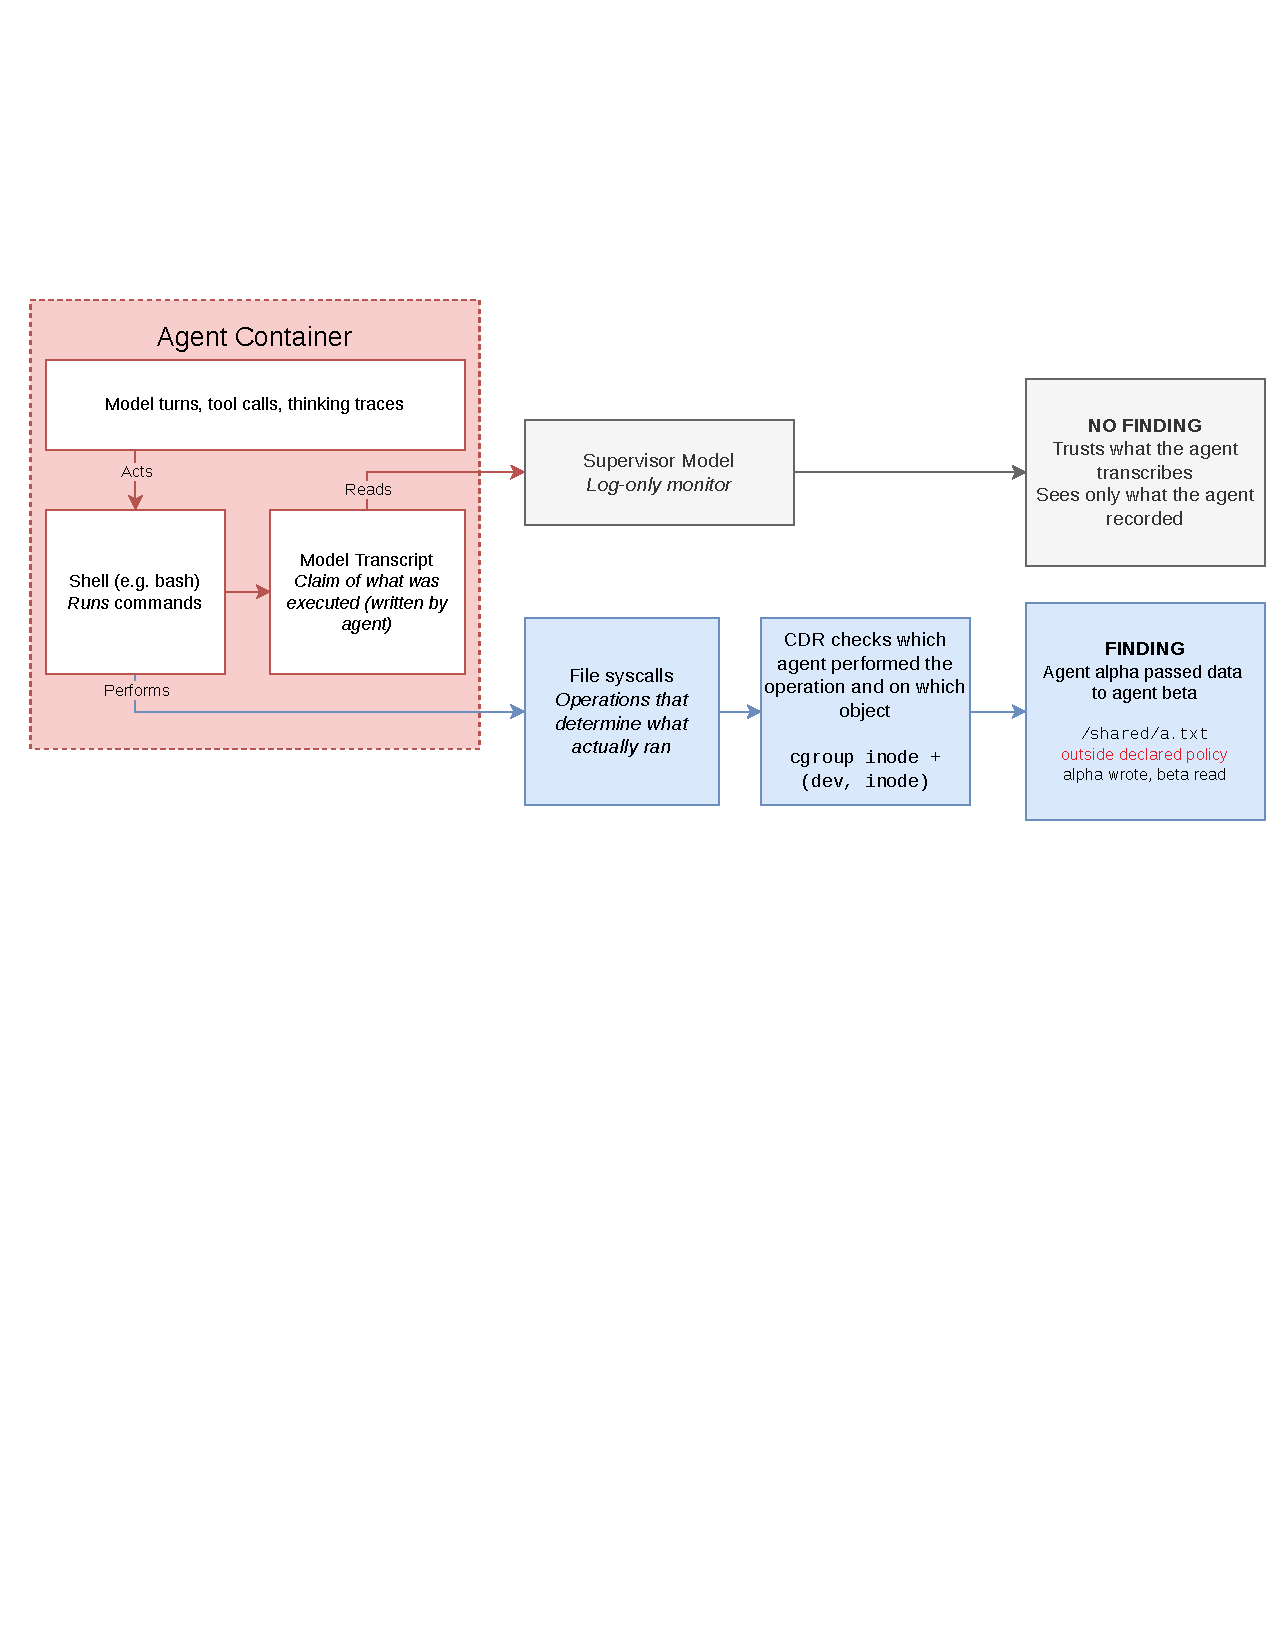
\includegraphics[width=\textwidth]{figures/fig1.pdf}
\caption{One action produces two records. Inside the dashed container everything is
written by the agent and can be rewritten by it, so the transcript is a claim; the
supervisor model has no input but that claim, and cannot separate a forged
transcript from an honest one that simply omits the action. The kernel witnesses
the syscall instead, resolves which agent performed the operation and on which
object, and emits an edge when two agents touch the same object. The object is
joined on device and inode, and the path is shown only for the reader. Agents
\texttt{alpha} and \texttt{beta} are two containers in one sandbox slice.}
\label{fig:trust}
\end{figure*}

Figure~\ref{fig:trust} summarises the arrangement the rest of this section builds.
Everything inside the dashed container is authored by the agent and can be
rewritten by it; everything outside is recorded by the kernel. The mechanism
exists so that a verdict depends only on the right-hand side, and every design
choice below is an attempt to move a piece of evidence across that boundary.

\1\noindent An agent is a cgroup v2 inode. The probe reads
\texttt{bpf\_get\_current\_cgroup\_id()} at syscall entry and resolves the caller
to the nearest registered cgroup in the sandbox slice, so identity is a property
of where the kernel placed the process rather than of anything the process
reports. A container-per-agent deployment needs no further configuration; several
agents inside one container are separable when the harness creates child cgroups
and declares them to the loader out of band. We first accepted any nested cgroup
whose name matched a prefix, and rejected it after review: an agent able to create
cgroups could adopt a neighbour's name, or create several identities and split its
own behaviour across them, which manufactures an edge between two halves of one
attacker. A name the subject chooses cannot be an identity, so declarations are
supplied by the deployment and nested cgroups that were not declared resolve to
their nearest declared ancestor.

\1\noindent Events are keyed on the pair
$(\mathit{device},\mathit{inode})$ rather than on the inode alone, because inode
numbers repeat across containers that share image layers. In our testbed the
shared volume collapses to a single key, $29/2693466$, for every agent, while the
same binary in three containers appears as inode $2604173$ under devices $85$,
$74$ and $82$. Keying on the inode would therefore report every agent that
launches \texttt{bash} as sharing an object with every other; keying on the pair
separates them without any knowledge of file names.

\1\noindent Ring-0 holds no per-syscall knowledge. For every syscall in
the slice the probe records the number, six registers, the cgroup, the command
name and up to two user strings, selected by a bitmap the loader derives at
startup from the kernel's own tracepoint metadata: an argument is marked when it
is typed \texttt{char~*} and its name indicates a path. Vectors such as
\texttt{execve} arguments are read element-wise onto a separate payload ring so
they are not truncated. Adding a syscall is a map insertion rather than a
recompilation. Syscalls outside the bitmap are counted in a per-agent histogram
rather than discarded, so an unmodelled channel surfaces as a frequency anomaly
against the benign baseline instead of as silence. Local sockets illustrate the
generality: the name of an \texttt{AF\_UNIX} endpoint lives behind a pointer to
a structure rather than in a path argument, so the probe reads the 2-byte address
family and follows \texttt{sun\_path} only when the family is \texttt{AF\_UNIX}.
No channel is enumerated anywhere in the code.

\1\noindent Paths reach the sensor as the agent wrote them. The loader
resolves them with \texttt{openat2} using \texttt{RESOLVE\_IN\_ROOT} and
\texttt{RESOLVE\_NO\_MAGICLINKS} against an \texttt{O\_PATH} descriptor for the
agent's \texttt{/proc/<pid>/root}, then \texttt{fstat}s the result. Both flags
exist because of observed failures: an absolute symlink target was otherwise
resolved against the host root, and \texttt{..} at the container root escaped to a
host inode shared by every container, and each produced false edges. Results are
cached per $(\mathit{agent},\mathit{path})$ and invalidated on \texttt{O\_CREAT},
since a delete-and-recreate can be served a different inode. Because \texttt{bind}
and \texttt{creat} create their object during the call, resolution at entry fails
by construction, so an event whose target does not yet exist is retried a bounded
number of times; a cached root that outlives its process falls back from the open
descriptor to the cached prefix and finally to the calling thread's own
\texttt{/proc/<tid>/root}.

\1\noindent The \texttt{sched\_process\_fork} tracepoint yields parent
and child, and \texttt{execve} yields the argument vector; together they form an
exec forest per agent. A declared tool call binds to the node whose effective
command matches it, after unwrapping one shell level and comparing basenames, and
that node's subtree is the delegated action. Every object touch carries a
thread-group identifier, so an edge can be walked back to the declaration that
authorised it. This is a containment claim rather than a proof: we can show that a
syscall fell inside the subtree a declaration authorised, not that the declaration
motivated it.

\1\noindent Declarations are reconciled against executions into four
classes: \texttt{match}, \texttt{mismatch} for a declaration with no execution,
\texttt{omission} for silence, and \texttt{surplus} for an execution with no
covering declaration. Separately, each edge is evaluated against a sanction set
over paths, yielding sanctioned or unsanctioned. Collusion is defined as an
unsanctioned edge. Syscalls are classified as mutators or sensors, and a syscall
we have not classified defaults to sense, because labelling a mutator as a sensor
and the reverse cost the same, so an unclassified verb participates as an
undirected adjacency rather than being dropped. The detector therefore records
what agents did and the policy decides whether it was permitted.


